%% Beamer-ported version of mru.tex ==
%% 
%% Original created 05-10-2008; ported to Beamer July 2025
\documentclass{beamer}

\usepackage{xcolor}
\usetheme{Copenhagen}  % Change to Madrid, Copenhagen, etc., for fancier look
% Define custom colors
\definecolor{electricblue}{RGB}{0,191,255} % Electric blue
\definecolor{creamyblue}{RGB}{173,216,230} % Creamy blue
\newcommand{\red}[1]{\textcolor{red}{#1}}
%\setbeamercolor{structure}{fg=electricblue} % Apply electric blue
\setbeamercolor{structure}{fg=creamyblue} % Uncomment for creamy blue

\usepackage[latin1]{inputenc}
\usepackage{amsmath}
\usepackage{cancel}
\usepackage{tikz}
\usepackage{xcolor}  % For colors and boxes
\usepackage{graphicx}  % For images

\hypersetup{
pdfpagemode={FullScreen},
pdftitle={MRU e12: ver1},
pdfauthor={mmatex},
pdfcreator={mmatex},
pdfproducer={mmatex},
pdfkeywords={Movimiento,Rectilineo,Uniforme}}

\def\psPi{3.14159265}

\input{lib/FORMULAS}
\input{lib/NOTASUNIDADES}



%________________________________________________________________(ult. col, 65)
% ==================== Titulo, autor, etc  ====================== 
\title{MRU e12: ver1}
\subtitle{MMaTeX - eScience}
\author{mmatex.com}
%________________________________________________________________(ult. col, 65)
%________________________________________________________________(ult. col, 65)



%%%%%%% Para pegar el log.. %%%%%%%%%%%%%%%%%%%%%%%%%%%%%%%
\logo{%
    \begin{tikzpicture}
        \node[opacity=0.2] {
\includegraphics[width=1cm]{images/citlogogrey.eps}};
    \end{tikzpicture}
}
%%%%%%%%%%%%%%%%%%%%%%%%%%%%%%%%%%%%%%%%%%%%%%%%%%%%%%%%%%%

\begin{document}

\maketitle







%________________________________________________________________(ult. col, 65)
% ========================== slide1 ============================= 
\begin{frame}
\frametitle{Movimiento Rectil\'ineo Uniforme}

% 
% -Paragraph1 
%----------------------------------------------------------------
%----------------------------------------------------------------
% -Idea1 
% ============================================================== 


La f\'ormula principal:

{\huge \vmru}

\vNUa
\end{frame}

\begin{frame}
\frametitle{MRU}
Recu\'erdalo por sus unidades:

\begin{equation*}
10\frac{\text{km}}{\text{h}} =
\frac{\text{Se recorren 10 km (\red{distancia})}}
{\text{en 1 hora (\red{tiempo})}}
\end{equation*}

Las otras dos f\'ormulas que se derivan de (\ref{vmru}) son:

{\large \xmru \\ \tmru}
% ============================================================== 
%----------------------------------------------------------------
%----------------------------------------------------------------
\end{frame}



%________________________________________________________________(ult. col, 65)
% ========================== slide2 ============================= 
\begin{frame}
\frametitle{MRU}

% 
% -Paragraph1 
%----------------------------------------------------------------
%----------------------------------------------------------------
% -Idea1 
% ============================================================== 
Es uniforme porque la velocidad no var\'ia en el tiempo; \\
(v es el mismo en cada unidad de tiempo!)

\begin{center}
\begin{tikzpicture}[scale=0.75]
\draw[->] (0,0) -- (8.5,0) node[below=0.5cm, midway] {t(s)};
\draw[->] (0,0) -- (0,4.5) node[left=0.5cm, midway, rotate=90] {v(cm/s)};
\draw[dashed] (0,2.5) -- (8.5,2.5);
\foreach \x in {1,2,3,4,5,6,7}
    \fill[red] (\x,2.5) circle (5pt);
\end{tikzpicture}
\end{center}

% ============================================================== 
%----------------------------------------------------------------
%----------------------------------------------------------------
\end{frame}



%________________________________________________________________(ult. col, 65)
% ========================== slide3 ============================= 
\begin{frame}
\frametitle{MRU}
% 
% -Paragraph1 
%----------------------------------------------------------------
%----------------------------------------------------------------
% -Idea1 
% ===============================================================
Un {{ objeto }} marcha 18 kilometros cada 6 minutos. 
\¿Qu\'e {{ distancia }} recorre al cabo de {{ 90 horas? }} %% Hay 1 elementos de distancia; Hay 2 elementos de tiempo; Hay 0 elementos de velocidad

\begin{itemize}
\item El 1er paso en la resoluci\'on de cualquier problema, es la
identificaci\'on de los elementos del problema.
\end{itemize}

\fcolorbox{black}{lightgray}{
\begin{tabular}{c}
{\bf Elementos del Problema}\\
$x=?$	\\
$v=\cancelto{3}{\frac{18}{6}}
\frac{kilometros}{minutos}$ \\
$t=90~horas$	\\
\end{tabular}
}

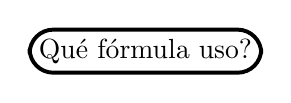
\begin{tikzpicture}
\node[draw, line width=0.5mm, rounded corners=3mm] at (8,2) {Qu\'e f\'ormula uso?};
\end{tikzpicture}

% ============================================================== 
%----------------------------------------------------------------
%----------------------------------------------------------------
\end{frame}



%________________________________________________________________(ult. col, 65)
% ========================== slide4 ============================= 
\begin{frame}
\frametitle{MRU}
% 
% -Paragraph1 
%----------------------------------------------------------------
%----------------------------------------------------------------
% -Idea1 
% ============================================================== 
{\huge \xmru}

Pero.. siempre debemos trabajar en el mismo sistema de unidades.
Es decir, si hay un metros/segundos,
debemos transformar los 
minutos a segundos :)

\begin{center}
\fcolorbox{red}{white}{
\parbox[c]{5cm}{
1 hora = 60 minutos \\
Entonces 90 horas son \\
90 $\times$ 60 minutos \\
90 horas =
5400 minutos.
}}
\end{center}

Finalmente..

% ============================================================== 
%----------------------------------------------------------------
%----------------------------------------------------------------
\end{frame}



%________________________________________________________________(ult. col, 65)
% ========================== slide5 ============================= 
\begin{frame}
\frametitle{MRU}
% 
% -Paragraph1 
%----------------------------------------------------------------
%----------------------------------------------------------------
% -Idea1 
% ============================================================== 
{\large
\begin{equation}
x=
\left(3\frac{\text{km}}{\cancel{\text{min}}}\right)
(5400\cancel{\text{min}})=
16200\text{ km}
\end{equation}}

% ============================================================== 
% -Idea2 
% ============================================================== 

La distancia que recorre el objeto es
\fbox{16200 km}

% ============================================================== 
%----------------------------------------------------------------
%----------------------------------------------------------------
\end{frame}




\end{document}
%%
%% End of Beamer-ported file ==
